\documentclass[twoside]{book}

% Packages required by doxygen
\usepackage{calc}
\usepackage{doxygen}
\usepackage{graphicx}
\usepackage[utf8]{inputenc}
\usepackage{makeidx}
\usepackage{multicol}
\usepackage{multirow}
\usepackage{textcomp}
\usepackage[table]{xcolor}

% Font selection
\usepackage[T1]{fontenc}
\usepackage{mathptmx}
\usepackage[scaled=.90]{helvet}
\usepackage{courier}
\usepackage{amssymb}
\usepackage{sectsty}
\renewcommand{\familydefault}{\sfdefault}
\allsectionsfont{%
  \fontseries{bc}\selectfont%
  \color{darkgray}%
}
\renewcommand{\DoxyLabelFont}{%
  \fontseries{bc}\selectfont%
  \color{darkgray}%
}

% Page & text layout
\usepackage{geometry}
\geometry{%
  a4paper,%
  top=2.5cm,%
  bottom=2.5cm,%
  left=2.5cm,%
  right=2.5cm%
}
\tolerance=750
\hfuzz=15pt
\hbadness=750
\setlength{\emergencystretch}{15pt}
\setlength{\parindent}{0cm}
\setlength{\parskip}{0.2cm}
\makeatletter
\renewcommand{\paragraph}{%
  \@startsection{paragraph}{4}{0ex}{-1.0ex}{1.0ex}{%
    \normalfont\normalsize\bfseries\SS@parafont%
  }%
}
\renewcommand{\subparagraph}{%
  \@startsection{subparagraph}{5}{0ex}{-1.0ex}{1.0ex}{%
    \normalfont\normalsize\bfseries\SS@subparafont%
  }%
}
\makeatother

% Headers & footers
\usepackage{fancyhdr}
\pagestyle{fancyplain}
\fancyhead[LE]{\fancyplain{}{\bfseries\thepage}}
\fancyhead[CE]{\fancyplain{}{}}
\fancyhead[RE]{\fancyplain{}{\bfseries\leftmark}}
\fancyhead[LO]{\fancyplain{}{\bfseries\rightmark}}
\fancyhead[CO]{\fancyplain{}{}}
\fancyhead[RO]{\fancyplain{}{\bfseries\thepage}}
\fancyfoot[LE]{\fancyplain{}{}}
\fancyfoot[CE]{\fancyplain{}{}}
\fancyfoot[RE]{\fancyplain{}{\bfseries\scriptsize Generated on Tue Jun 19 2018 20\-:58\-:24 for leistungsnachweis-\/cas by Doxygen }}
\fancyfoot[LO]{\fancyplain{}{\bfseries\scriptsize Generated on Tue Jun 19 2018 20\-:58\-:24 for leistungsnachweis-\/cas by Doxygen }}
\fancyfoot[CO]{\fancyplain{}{}}
\fancyfoot[RO]{\fancyplain{}{}}
\renewcommand{\footrulewidth}{0.4pt}
\renewcommand{\chaptermark}[1]{%
  \markboth{#1}{}%
}
\renewcommand{\sectionmark}[1]{%
  \markright{\thesection\ #1}%
}

% Indices & bibliography
\usepackage{natbib}
\usepackage[titles]{tocloft}
\setcounter{tocdepth}{3}
\setcounter{secnumdepth}{5}
\makeindex

% Hyperlinks (required, but should be loaded last)
\usepackage{ifpdf}
\ifpdf
  \usepackage[pdftex,pagebackref=true]{hyperref}
\else
  \usepackage[ps2pdf,pagebackref=true]{hyperref}
\fi
\hypersetup{%
  colorlinks=true,%
  linkcolor=blue,%
  citecolor=blue,%
  unicode%
}

% Custom commands
\newcommand{\clearemptydoublepage}{%
  \newpage{\pagestyle{empty}\cleardoublepage}%
}


%===== C O N T E N T S =====

\begin{document}

% Titlepage & ToC
\hypersetup{pageanchor=false}
\pagenumbering{roman}
\begin{titlepage}
\vspace*{7cm}
\begin{center}%
{\Large leistungsnachweis-\/cas }\\
\vspace*{1cm}
{\large Generated by Doxygen 1.8.6}\\
\vspace*{0.5cm}
{\small Tue Jun 19 2018 20:58:24}\\
\end{center}
\end{titlepage}
\clearemptydoublepage
\tableofcontents
\clearemptydoublepage
\pagenumbering{arabic}
\hypersetup{pageanchor=true}

%--- Begin generated contents ---
\chapter{Hierarchical Index}
\section{Class Hierarchy}
This inheritance list is sorted roughly, but not completely, alphabetically\-:\begin{DoxyCompactList}
\item binary\-\_\-function\begin{DoxyCompactList}
\item \contentsline{section}{Lab\-Graph\-:\-:Edge\-:\-:Compare\-Edges}{\pageref{struct_lab_graph_1_1_edge_1_1_compare_edges}}{}
\end{DoxyCompactList}
\item \contentsline{section}{Cell}{\pageref{struct_cell}}{}
\item \contentsline{section}{Lab\-Graph}{\pageref{class_lab_graph}}{}
\item \contentsline{section}{Recursive\-Backtracker}{\pageref{class_recursive_backtracker}}{}
\item \contentsline{section}{Recursive\-Division}{\pageref{class_recursive_division}}{}
\end{DoxyCompactList}

\chapter{Class Index}
\section{Class List}
Here are the classes, structs, unions and interfaces with brief descriptions\-:\begin{DoxyCompactList}
\item\contentsline{section}{\hyperlink{struct_cell}{Cell} }{\pageref{struct_cell}}{}
\item\contentsline{section}{\hyperlink{struct_lab_graph_1_1_edge_1_1_compare_edges}{Lab\-Graph\-::\-Edge\-::\-Compare\-Edges} }{\pageref{struct_lab_graph_1_1_edge_1_1_compare_edges}}{}
\item\contentsline{section}{\hyperlink{class_lab_graph}{Lab\-Graph} }{\pageref{class_lab_graph}}{}
\item\contentsline{section}{\hyperlink{class_recursive_backtracker}{Recursive\-Backtracker} }{\pageref{class_recursive_backtracker}}{}
\item\contentsline{section}{\hyperlink{class_recursive_division}{Recursive\-Division} }{\pageref{class_recursive_division}}{}
\end{DoxyCompactList}

\chapter{Class Documentation}
\hypertarget{struct_cell}{\section{Cell Struct Reference}
\label{struct_cell}\index{Cell@{Cell}}
}
\subsection*{Public Attributes}
\begin{DoxyCompactItemize}
\item 
\hypertarget{struct_cell_aa432bd8a7ea643f6aad4e1ebc27e2b2d}{char {\bfseries directions}}\label{struct_cell_aa432bd8a7ea643f6aad4e1ebc27e2b2d}

\item 
\hypertarget{struct_cell_ac008158796a0bfdf37be2f26eff651ef}{int {\bfseries x}}\label{struct_cell_ac008158796a0bfdf37be2f26eff651ef}

\item 
\hypertarget{struct_cell_ab99a0cead05c6b8129ddf3231b11c1ad}{int {\bfseries y}}\label{struct_cell_ab99a0cead05c6b8129ddf3231b11c1ad}

\item 
\hypertarget{struct_cell_ac5ec3ea991a8936c0c086803158e8903}{void $\ast$ {\bfseries parent\-Cell}}\label{struct_cell_ac5ec3ea991a8936c0c086803158e8903}

\item 
\hypertarget{struct_cell_ad7cbb10d42690e0e3d566456899d8204}{char {\bfseries image}}\label{struct_cell_ad7cbb10d42690e0e3d566456899d8204}

\end{DoxyCompactItemize}


The documentation for this struct was generated from the following file\-:\begin{DoxyCompactItemize}
\item 
recursive\-Backtracker/Recursive\-Backtracker.\-h\end{DoxyCompactItemize}

\hypertarget{struct_lab_graph_1_1_edge_1_1_compare_edges}{\section{Lab\-Graph\-:\-:Edge\-:\-:Compare\-Edges Struct Reference}
\label{struct_lab_graph_1_1_edge_1_1_compare_edges}\index{Lab\-Graph\-::\-Edge\-::\-Compare\-Edges@{Lab\-Graph\-::\-Edge\-::\-Compare\-Edges}}
}


{\ttfamily \#include $<$Lab\-Graph.\-h$>$}

Inheritance diagram for Lab\-Graph\-:\-:Edge\-:\-:Compare\-Edges\-:\begin{figure}[H]
\begin{center}
\leavevmode
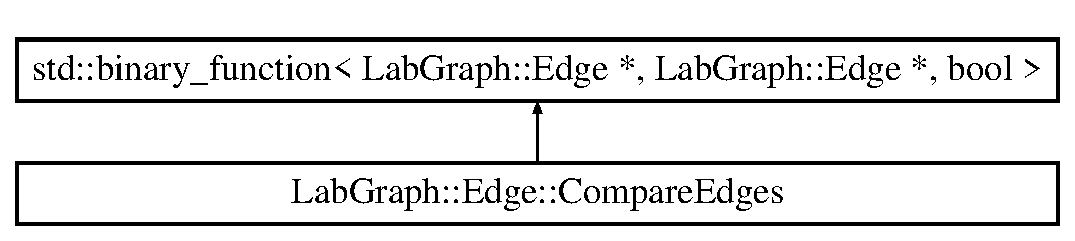
\includegraphics[height=2.000000cm]{struct_lab_graph_1_1_edge_1_1_compare_edges}
\end{center}
\end{figure}
\subsection*{Public Member Functions}
\begin{DoxyCompactItemize}
\item 
\hypertarget{struct_lab_graph_1_1_edge_1_1_compare_edges_a90996d6326dc05c6536d8205e16ca437}{bool {\bfseries operator()} (const Lab\-Graph\-::\-Edge $\ast$lhs, const Lab\-Graph\-::\-Edge $\ast$rhs) const }\label{struct_lab_graph_1_1_edge_1_1_compare_edges_a90996d6326dc05c6536d8205e16ca437}

\end{DoxyCompactItemize}


\subsection{Detailed Description}
Compare function for two edges. Compares two edges by weight. Needed to manage edgepointers in a priority queue. 

The documentation for this struct was generated from the following file\-:\begin{DoxyCompactItemize}
\item 
prims/Lab\-Graph.\-h\end{DoxyCompactItemize}

\hypertarget{class_lab_graph}{\section{Lab\-Graph Class Reference}
\label{class_lab_graph}\index{Lab\-Graph@{Lab\-Graph}}
}
\subsection*{Public Member Functions}
\begin{DoxyCompactItemize}
\item 
\hyperlink{class_lab_graph_aa10dea2f824ce99b6175952650ea7349}{Lab\-Graph} (int height, int width)
\item 
\hyperlink{class_lab_graph_ac37389ef1300ceb90c81fc482971471f}{$\sim$\-Lab\-Graph} ()
\item 
void \hyperlink{class_lab_graph_ab54dc4e91349cfeca4e501ab7bd340af}{init\-Graph} ()
\item 
void \hyperlink{class_lab_graph_ab9767076b66b28dae3c47b9c3177b498}{build\-Lab\-With\-Prim} ()
\item 
void \hyperlink{class_lab_graph_a04d781d9fe079eef7374babe6318c498}{build\-Lab\-With\-Rec\-Bac} ()
\item 
void \hyperlink{class_lab_graph_a478f4acb3c4da8d81b079d26d83c9f42}{graph\-To\-Pic} (string format)
\item 
void \hyperlink{class_lab_graph_afca83817aa9ca4996f49fbd2dd2618f5}{make\-Video} ()
\item 
void \hyperlink{class_lab_graph_a1b88384d6363809ae16384205ecff4e2}{set\-Lab} (bool $\ast$$\ast$)
\item 
void \hyperlink{class_lab_graph_a44653d0495a05c3ba03e661d342b15e7}{set\-Dimensions} (int, int)
\item 
void \hyperlink{class_lab_graph_a5a9e4661d1b03a3de1e7b669ba9aa8e5}{easy\-Test} ()
\end{DoxyCompactItemize}
\subsection*{Friends}
\begin{DoxyCompactItemize}
\item 
std\-::ostream \& \hyperlink{class_lab_graph_a98ed4ce18d06e538a4ef79d43997a19f}{operator$<$$<$} (std\-::ostream \&, const \hyperlink{class_lab_graph}{Lab\-Graph} \&)
\end{DoxyCompactItemize}


\subsection{Constructor \& Destructor Documentation}
\hypertarget{class_lab_graph_aa10dea2f824ce99b6175952650ea7349}{\index{Lab\-Graph@{Lab\-Graph}!Lab\-Graph@{Lab\-Graph}}
\index{Lab\-Graph@{Lab\-Graph}!LabGraph@{Lab\-Graph}}
\subsubsection[{Lab\-Graph}]{\setlength{\rightskip}{0pt plus 5cm}Lab\-Graph\-::\-Lab\-Graph (
\begin{DoxyParamCaption}
\item[{int}]{height, }
\item[{int}]{width}
\end{DoxyParamCaption}
)}}\label{class_lab_graph_aa10dea2f824ce99b6175952650ea7349}
Constructor. 
\begin{DoxyParams}{Parameters}
{\em height} & Height of the graph. \\
\hline
{\em width} & Width of the graph. \\
\hline
\end{DoxyParams}
\hypertarget{class_lab_graph_ac37389ef1300ceb90c81fc482971471f}{\index{Lab\-Graph@{Lab\-Graph}!$\sim$\-Lab\-Graph@{$\sim$\-Lab\-Graph}}
\index{$\sim$\-Lab\-Graph@{$\sim$\-Lab\-Graph}!LabGraph@{Lab\-Graph}}
\subsubsection[{$\sim$\-Lab\-Graph}]{\setlength{\rightskip}{0pt plus 5cm}Lab\-Graph\-::$\sim$\-Lab\-Graph (
\begin{DoxyParamCaption}
{}
\end{DoxyParamCaption}
)\hspace{0.3cm}{\ttfamily [default]}}}\label{class_lab_graph_ac37389ef1300ceb90c81fc482971471f}
Destructor of the graph. 

\subsection{Member Function Documentation}
\hypertarget{class_lab_graph_ab9767076b66b28dae3c47b9c3177b498}{\index{Lab\-Graph@{Lab\-Graph}!build\-Lab\-With\-Prim@{build\-Lab\-With\-Prim}}
\index{build\-Lab\-With\-Prim@{build\-Lab\-With\-Prim}!LabGraph@{Lab\-Graph}}
\subsubsection[{build\-Lab\-With\-Prim}]{\setlength{\rightskip}{0pt plus 5cm}void Lab\-Graph\-::build\-Lab\-With\-Prim (
\begin{DoxyParamCaption}
{}
\end{DoxyParamCaption}
)}}\label{class_lab_graph_ab9767076b66b28dae3c47b9c3177b498}
Creates a Labyrinth on the Graph with prims algorithm. \hypertarget{class_lab_graph_a04d781d9fe079eef7374babe6318c498}{\index{Lab\-Graph@{Lab\-Graph}!build\-Lab\-With\-Rec\-Bac@{build\-Lab\-With\-Rec\-Bac}}
\index{build\-Lab\-With\-Rec\-Bac@{build\-Lab\-With\-Rec\-Bac}!LabGraph@{Lab\-Graph}}
\subsubsection[{build\-Lab\-With\-Rec\-Bac}]{\setlength{\rightskip}{0pt plus 5cm}void Lab\-Graph\-::build\-Lab\-With\-Rec\-Bac (
\begin{DoxyParamCaption}
{}
\end{DoxyParamCaption}
)}}\label{class_lab_graph_a04d781d9fe079eef7374babe6318c498}
Creates a Labyrinth on the Graph with recursive backtracing algorithm. \hypertarget{class_lab_graph_a5a9e4661d1b03a3de1e7b669ba9aa8e5}{\index{Lab\-Graph@{Lab\-Graph}!easy\-Test@{easy\-Test}}
\index{easy\-Test@{easy\-Test}!LabGraph@{Lab\-Graph}}
\subsubsection[{easy\-Test}]{\setlength{\rightskip}{0pt plus 5cm}void Lab\-Graph\-::easy\-Test (
\begin{DoxyParamCaption}
{}
\end{DoxyParamCaption}
)}}\label{class_lab_graph_a5a9e4661d1b03a3de1e7b669ba9aa8e5}
Once a simple test method this became the starter\-:). \hypertarget{class_lab_graph_a478f4acb3c4da8d81b079d26d83c9f42}{\index{Lab\-Graph@{Lab\-Graph}!graph\-To\-Pic@{graph\-To\-Pic}}
\index{graph\-To\-Pic@{graph\-To\-Pic}!LabGraph@{Lab\-Graph}}
\subsubsection[{graph\-To\-Pic}]{\setlength{\rightskip}{0pt plus 5cm}void Lab\-Graph\-::graph\-To\-Pic (
\begin{DoxyParamCaption}
\item[{string}]{format}
\end{DoxyParamCaption}
)}}\label{class_lab_graph_a478f4acb3c4da8d81b079d26d83c9f42}
Creates a picture of the current graph using graphviz. 
\begin{DoxyParams}{Parameters}
{\em format} & Outputformat of the picture e.\-g. \char`\"{}jpg\char`\"{} \char`\"{}png\char`\"{}... \\
\hline
\end{DoxyParams}
\hypertarget{class_lab_graph_ab54dc4e91349cfeca4e501ab7bd340af}{\index{Lab\-Graph@{Lab\-Graph}!init\-Graph@{init\-Graph}}
\index{init\-Graph@{init\-Graph}!LabGraph@{Lab\-Graph}}
\subsubsection[{init\-Graph}]{\setlength{\rightskip}{0pt plus 5cm}void Lab\-Graph\-::init\-Graph (
\begin{DoxyParamCaption}
{}
\end{DoxyParamCaption}
)}}\label{class_lab_graph_ab54dc4e91349cfeca4e501ab7bd340af}
Creates a square with heigt x width nodes connected by edges. \hypertarget{class_lab_graph_afca83817aa9ca4996f49fbd2dd2618f5}{\index{Lab\-Graph@{Lab\-Graph}!make\-Video@{make\-Video}}
\index{make\-Video@{make\-Video}!LabGraph@{Lab\-Graph}}
\subsubsection[{make\-Video}]{\setlength{\rightskip}{0pt plus 5cm}void Lab\-Graph\-::make\-Video (
\begin{DoxyParamCaption}
{}
\end{DoxyParamCaption}
)}}\label{class_lab_graph_afca83817aa9ca4996f49fbd2dd2618f5}
Makes a video of the graph creation. \hypertarget{class_lab_graph_a44653d0495a05c3ba03e661d342b15e7}{\index{Lab\-Graph@{Lab\-Graph}!set\-Dimensions@{set\-Dimensions}}
\index{set\-Dimensions@{set\-Dimensions}!LabGraph@{Lab\-Graph}}
\subsubsection[{set\-Dimensions}]{\setlength{\rightskip}{0pt plus 5cm}void Lab\-Graph\-::set\-Dimensions (
\begin{DoxyParamCaption}
\item[{int}]{x, }
\item[{int}]{y}
\end{DoxyParamCaption}
)}}\label{class_lab_graph_a44653d0495a05c3ba03e661d342b15e7}
Can only be used on an uninizialized graph. Sets the height and width and initializes the graph. This is used to diplay the labyrinth created by recursive division. \hypertarget{class_lab_graph_a1b88384d6363809ae16384205ecff4e2}{\index{Lab\-Graph@{Lab\-Graph}!set\-Lab@{set\-Lab}}
\index{set\-Lab@{set\-Lab}!LabGraph@{Lab\-Graph}}
\subsubsection[{set\-Lab}]{\setlength{\rightskip}{0pt plus 5cm}void Lab\-Graph\-::set\-Lab (
\begin{DoxyParamCaption}
\item[{bool $\ast$$\ast$}]{bool\-Array}
\end{DoxyParamCaption}
)}}\label{class_lab_graph_a1b88384d6363809ae16384205ecff4e2}
Sets the color of all edges to black or white. This is used to diplay the labyrinth created by recursive division. 

\subsection{Friends And Related Function Documentation}
\hypertarget{class_lab_graph_a98ed4ce18d06e538a4ef79d43997a19f}{\index{Lab\-Graph@{Lab\-Graph}!operator$<$$<$@{operator$<$$<$}}
\index{operator$<$$<$@{operator$<$$<$}!LabGraph@{Lab\-Graph}}
\subsubsection[{operator$<$$<$}]{\setlength{\rightskip}{0pt plus 5cm}std\-::ostream\& operator$<$$<$ (
\begin{DoxyParamCaption}
\item[{std\-::ostream \&}]{os, }
\item[{const {\bf Lab\-Graph} \&}]{graph}
\end{DoxyParamCaption}
)\hspace{0.3cm}{\ttfamily [friend]}}}\label{class_lab_graph_a98ed4ce18d06e538a4ef79d43997a19f}
Outputs the graph in D\-O\-T-\/form so it can be interpreted by graphviz. \begin{DoxyReturn}{Returns}

\end{DoxyReturn}


The documentation for this class was generated from the following files\-:\begin{DoxyCompactItemize}
\item 
prims/Lab\-Graph.\-h\item 
prims/Lab\-Graph.\-cpp\end{DoxyCompactItemize}

\hypertarget{class_recursive_backtracker}{\section{Recursive\-Backtracker Class Reference}
\label{class_recursive_backtracker}\index{Recursive\-Backtracker@{Recursive\-Backtracker}}
}
\subsection*{Public Member Functions}
\begin{DoxyCompactItemize}
\item 
int \hyperlink{class_recursive_backtracker_a114ae44592829d9ddd93f82985ac8cc3}{init\-Maze} ()
\item 
\hyperlink{struct_cell}{Cell} $\ast$ \hyperlink{class_recursive_backtracker_a9840a665c1569cc03d920dd92d883d87}{backtracking} (\hyperlink{struct_cell}{Cell} $\ast$c)
\item 
void \hyperlink{class_recursive_backtracker_af05c0897809de82fccdd276433f9aee7}{draw\-Maze} ()
\item 
\hypertarget{class_recursive_backtracker_a8f3059326aaee4f41b56d2f6efecfc11}{int {\bfseries start\-Maze} ()}\label{class_recursive_backtracker_a8f3059326aaee4f41b56d2f6efecfc11}

\item 
\hypertarget{class_recursive_backtracker_a78194dbc1284dbe435d87c5158491dcd}{double {\bfseries test\-Method} ()}\label{class_recursive_backtracker_a78194dbc1284dbe435d87c5158491dcd}

\end{DoxyCompactItemize}


\subsection{Member Function Documentation}
\hypertarget{class_recursive_backtracker_a9840a665c1569cc03d920dd92d883d87}{\index{Recursive\-Backtracker@{Recursive\-Backtracker}!backtracking@{backtracking}}
\index{backtracking@{backtracking}!RecursiveBacktracker@{Recursive\-Backtracker}}
\subsubsection[{backtracking}]{\setlength{\rightskip}{0pt plus 5cm}{\bf Cell} $\ast$ Recursive\-Backtracker\-::backtracking (
\begin{DoxyParamCaption}
\item[{{\bf Cell} $\ast$}]{n}
\end{DoxyParamCaption}
)}}\label{class_recursive_backtracker_a9840a665c1569cc03d920dd92d883d87}
removes the wall between the two cells and marks the new cell as visited. this continues until a cell that has no unvisited neighbours is reached \hypertarget{class_recursive_backtracker_af05c0897809de82fccdd276433f9aee7}{\index{Recursive\-Backtracker@{Recursive\-Backtracker}!draw\-Maze@{draw\-Maze}}
\index{draw\-Maze@{draw\-Maze}!RecursiveBacktracker@{Recursive\-Backtracker}}
\subsubsection[{draw\-Maze}]{\setlength{\rightskip}{0pt plus 5cm}void Recursive\-Backtracker\-::draw\-Maze (
\begin{DoxyParamCaption}
{}
\end{DoxyParamCaption}
)}}\label{class_recursive_backtracker_af05c0897809de82fccdd276433f9aee7}
Created by Anja Wimmer on 27.\-04.\-18. Quelle\-: (\href{https://en.wikipedia.org/wiki/Maze_generation_algorithm#Recursive_backtracker}{\tt https\-://en.\-wikipedia.\-org/wiki/\-Maze\-\_\-generation\-\_\-algorithm\#\-Recursive\-\_\-backtracker})print maze to terminal \hypertarget{class_recursive_backtracker_a114ae44592829d9ddd93f82985ac8cc3}{\index{Recursive\-Backtracker@{Recursive\-Backtracker}!init\-Maze@{init\-Maze}}
\index{init\-Maze@{init\-Maze}!RecursiveBacktracker@{Recursive\-Backtracker}}
\subsubsection[{init\-Maze}]{\setlength{\rightskip}{0pt plus 5cm}int Recursive\-Backtracker\-::init\-Maze (
\begin{DoxyParamCaption}
{}
\end{DoxyParamCaption}
)}}\label{class_recursive_backtracker_a114ae44592829d9ddd93f82985ac8cc3}
large grid of cells, each cell starting with four walls \begin{DoxyReturn}{Returns}

\end{DoxyReturn}


The documentation for this class was generated from the following files\-:\begin{DoxyCompactItemize}
\item 
recursive\-Backtracker/Recursive\-Backtracker.\-h\item 
recursive\-Backtracker/Recursive\-Backtracker.\-cpp\end{DoxyCompactItemize}

\hypertarget{class_recursive_division}{\section{Recursive\-Division Class Reference}
\label{class_recursive_division}\index{Recursive\-Division@{Recursive\-Division}}
}


{\ttfamily \#include $<$Recursive\-Division.\-h$>$}

\subsection*{Public Member Functions}
\begin{DoxyCompactItemize}
\item 
bool $\ast$$\ast$ \hyperlink{class_recursive_division_a3572b23c6eb7d255d1810efe2e40687f}{init\-Maze} (int width, int height)
\item 
int \hyperlink{class_recursive_division_a09758db0100db2aa3902535869ba7d7c}{generate\-Maze} (std\-::istream \&is)
\item 
void \hyperlink{class_recursive_division_a38669e9dcfc8e9056928333613adbaa1}{divide\-Field} (bool $\ast$$\ast$field, int left, int right, int top, int bottom)
\item 
void \hyperlink{class_recursive_division_a16e56a56f3d84644211cff7844c3b4b8}{divide\-Vertical} (bool $\ast$$\ast$field, int left, int right, int top, int bottom)
\item 
void \hyperlink{class_recursive_division_a2d4bb0a2bd69216c35b27e8448e4b1af}{divide\-Horizontal} (bool $\ast$$\ast$field, int left, int right, int top, int bottom)
\item 
void \hyperlink{class_recursive_division_a22f4a67b74499117e6d38cb2de49b9c6}{make\-Maze\-Opening} (bool $\ast$$\ast$field, int rows, int cols)
\item 
void \hyperlink{class_recursive_division_a16d033f98dd8d407d7ccf4828b3391e7}{draw\-Maze} (bool $\ast$$\ast$field, std\-::ostream \&output)
\item 
int \hyperlink{class_recursive_division_aba7306d64093888306f2479fd3e629e6}{generate\-Random\-Int} (int lower, int upper)
\item 
bool \hyperlink{class_recursive_division_a64a45071f78e79f4edd29578d92388e0}{generate\-Random\-Boolean} ()
\end{DoxyCompactItemize}
\subsection*{Public Attributes}
\begin{DoxyCompactItemize}
\item 
\hyperlink{class_lab_graph}{Lab\-Graph} $\ast$ \hyperlink{class_recursive_division_ac2402e5bb64bd4444f584ac6b237f84b}{lab\-Printer}
\item 
bool \hyperlink{class_recursive_division_a3ee7d465c3a8637c37a08de75ced22c1}{debug\-Mode} = false
\end{DoxyCompactItemize}


\subsection{Detailed Description}
Class with recursive division algorithm.

Creates a Nx\-M empty maze field surrounded by a wall. Each time this field will be separated by a wall with a passage into two smaller fields. These new small field will be separated in another two smaller fields and so on.

After each field have the minimum size of 2x2 a start opening and a end opening will be calculated. 

\subsection{Member Function Documentation}
\hypertarget{class_recursive_division_a38669e9dcfc8e9056928333613adbaa1}{\index{Recursive\-Division@{Recursive\-Division}!divide\-Field@{divide\-Field}}
\index{divide\-Field@{divide\-Field}!RecursiveDivision@{Recursive\-Division}}
\subsubsection[{divide\-Field}]{\setlength{\rightskip}{0pt plus 5cm}void Recursive\-Division\-::divide\-Field (
\begin{DoxyParamCaption}
\item[{bool $\ast$$\ast$}]{field, }
\item[{int}]{left, }
\item[{int}]{right, }
\item[{int}]{top, }
\item[{int}]{bottom}
\end{DoxyParamCaption}
)}}\label{class_recursive_division_a38669e9dcfc8e9056928333613adbaa1}
Arbitrator method for the recursive division.

It consumes the maze and the current coordinates of the field. These coordinates are the four directions. This method choose by the width and height if the field will be divided and in which direction. 
\begin{DoxyParams}{Parameters}
{\em field} & The complete maze field. \\
\hline
{\em left} & The column index of the left column. \\
\hline
{\em right} & The column index of the right column. \\
\hline
{\em top} & The row index of the top row. \\
\hline
{\em bottom} & The row index of the bottom row. \\
\hline
\end{DoxyParams}
\hypertarget{class_recursive_division_a2d4bb0a2bd69216c35b27e8448e4b1af}{\index{Recursive\-Division@{Recursive\-Division}!divide\-Horizontal@{divide\-Horizontal}}
\index{divide\-Horizontal@{divide\-Horizontal}!RecursiveDivision@{Recursive\-Division}}
\subsubsection[{divide\-Horizontal}]{\setlength{\rightskip}{0pt plus 5cm}void Recursive\-Division\-::divide\-Horizontal (
\begin{DoxyParamCaption}
\item[{bool $\ast$$\ast$}]{field, }
\item[{int}]{left, }
\item[{int}]{right, }
\item[{int}]{top, }
\item[{int}]{bottom}
\end{DoxyParamCaption}
)}}\label{class_recursive_division_a2d4bb0a2bd69216c35b27e8448e4b1af}
Divide the sub-\/field with a horizontal wall.

It choose a random number for the column index where the wall will be placed. After that the wall will be added and a random column index is calculated to open the passage. After that, this method calls the \hyperlink{class_recursive_division_a09758db0100db2aa3902535869ba7d7c}{generate\-Maze()} Method again with the new two, smaller fields. 
\begin{DoxyParams}{Parameters}
{\em field} & The complete maze field. \\
\hline
{\em left} & The column index of the left column. \\
\hline
{\em right} & The column index of the right column. \\
\hline
{\em top} & The row index of the top row. \\
\hline
{\em bottom} & The row index of the bottom row. \\
\hline
\end{DoxyParams}
\hypertarget{class_recursive_division_a16e56a56f3d84644211cff7844c3b4b8}{\index{Recursive\-Division@{Recursive\-Division}!divide\-Vertical@{divide\-Vertical}}
\index{divide\-Vertical@{divide\-Vertical}!RecursiveDivision@{Recursive\-Division}}
\subsubsection[{divide\-Vertical}]{\setlength{\rightskip}{0pt plus 5cm}void Recursive\-Division\-::divide\-Vertical (
\begin{DoxyParamCaption}
\item[{bool $\ast$$\ast$}]{field, }
\item[{int}]{left, }
\item[{int}]{right, }
\item[{int}]{top, }
\item[{int}]{bottom}
\end{DoxyParamCaption}
)}}\label{class_recursive_division_a16e56a56f3d84644211cff7844c3b4b8}
Divide the sub-\/field with a vertical wall.

It choose a random number for the row index where the wall will be placed. After that the wall will be added and a random row index is calculated to open the passage. After that, this method calls the \hyperlink{class_recursive_division_a09758db0100db2aa3902535869ba7d7c}{generate\-Maze()} Method again with the new two, smaller fields. 
\begin{DoxyParams}{Parameters}
{\em field} & The complete maze field. \\
\hline
{\em left} & The column index of the left column. \\
\hline
{\em right} & The column index of the right column. \\
\hline
{\em top} & The row index of the top row. \\
\hline
{\em bottom} & The row index of the bottom row. \\
\hline
\end{DoxyParams}
\hypertarget{class_recursive_division_a16d033f98dd8d407d7ccf4828b3391e7}{\index{Recursive\-Division@{Recursive\-Division}!draw\-Maze@{draw\-Maze}}
\index{draw\-Maze@{draw\-Maze}!RecursiveDivision@{Recursive\-Division}}
\subsubsection[{draw\-Maze}]{\setlength{\rightskip}{0pt plus 5cm}void Recursive\-Division\-::draw\-Maze (
\begin{DoxyParamCaption}
\item[{bool $\ast$$\ast$}]{field, }
\item[{std\-::ostream \&}]{output}
\end{DoxyParamCaption}
)}}\label{class_recursive_division_a16d033f98dd8d407d7ccf4828b3391e7}
Consumes the maze field and draw it at the console output. 
\begin{DoxyParams}{Parameters}
{\em field} & Maze field. \\
\hline
{\em output} & output stream (only for testing purpose). \\
\hline
\end{DoxyParams}
\hypertarget{class_recursive_division_a09758db0100db2aa3902535869ba7d7c}{\index{Recursive\-Division@{Recursive\-Division}!generate\-Maze@{generate\-Maze}}
\index{generate\-Maze@{generate\-Maze}!RecursiveDivision@{Recursive\-Division}}
\subsubsection[{generate\-Maze}]{\setlength{\rightskip}{0pt plus 5cm}int Recursive\-Division\-::generate\-Maze (
\begin{DoxyParamCaption}
\item[{std\-::istream \&}]{is}
\end{DoxyParamCaption}
)}}\label{class_recursive_division_a09758db0100db2aa3902535869ba7d7c}
Start method of this class with console.

It ask for cols and rows of the maze. Theses are the relative sizes of the maze, because of the walls. A maze with 2 cols have an absolute width of 6. Two for the walls on the left and on the right, two for the given col amount and 2 for walls between them. 
\begin{DoxyParams}{Parameters}
{\em is} & input-\/stream for reading input params. \\
\hline
\end{DoxyParams}
\begin{DoxyReturn}{Returns}
0 if no exception occurs. 
\end{DoxyReturn}
Enable Debug mode for maze printing\-:\hypertarget{class_recursive_division_a64a45071f78e79f4edd29578d92388e0}{\index{Recursive\-Division@{Recursive\-Division}!generate\-Random\-Boolean@{generate\-Random\-Boolean}}
\index{generate\-Random\-Boolean@{generate\-Random\-Boolean}!RecursiveDivision@{Recursive\-Division}}
\subsubsection[{generate\-Random\-Boolean}]{\setlength{\rightskip}{0pt plus 5cm}bool Recursive\-Division\-::generate\-Random\-Boolean (
\begin{DoxyParamCaption}
{}
\end{DoxyParamCaption}
)}}\label{class_recursive_division_a64a45071f78e79f4edd29578d92388e0}
Generate a random boolean value. \begin{DoxyReturn}{Returns}
random true or false. 
\end{DoxyReturn}
\hypertarget{class_recursive_division_aba7306d64093888306f2479fd3e629e6}{\index{Recursive\-Division@{Recursive\-Division}!generate\-Random\-Int@{generate\-Random\-Int}}
\index{generate\-Random\-Int@{generate\-Random\-Int}!RecursiveDivision@{Recursive\-Division}}
\subsubsection[{generate\-Random\-Int}]{\setlength{\rightskip}{0pt plus 5cm}int Recursive\-Division\-::generate\-Random\-Int (
\begin{DoxyParamCaption}
\item[{int}]{lower, }
\item[{int}]{upper}
\end{DoxyParamCaption}
)}}\label{class_recursive_division_aba7306d64093888306f2479fd3e629e6}
Generate a random integer value between the lower and the upper boundary. 
\begin{DoxyParams}{Parameters}
{\em lower} & Lower bound. \\
\hline
{\em upper} & Upper bound. \\
\hline
\end{DoxyParams}
\begin{DoxyReturn}{Returns}
random value. 
\end{DoxyReturn}
\hypertarget{class_recursive_division_a3572b23c6eb7d255d1810efe2e40687f}{\index{Recursive\-Division@{Recursive\-Division}!init\-Maze@{init\-Maze}}
\index{init\-Maze@{init\-Maze}!RecursiveDivision@{Recursive\-Division}}
\subsubsection[{init\-Maze}]{\setlength{\rightskip}{0pt plus 5cm}bool $\ast$$\ast$ Recursive\-Division\-::init\-Maze (
\begin{DoxyParamCaption}
\item[{int}]{width, }
\item[{int}]{height}
\end{DoxyParamCaption}
)}}\label{class_recursive_division_a3572b23c6eb7d255d1810efe2e40687f}
Method which generate the empty maze field.

Field is surrounded by a wall.

The generated field is a 2\-D -\/ boolean array. 
\begin{DoxyParams}{Parameters}
{\em width} & Absolute width of the maze. \\
\hline
{\em height} & Absolute height of the maze. \\
\hline
\end{DoxyParams}
\begin{DoxyReturn}{Returns}
The generated maze field as 2\-D bool array. 
\end{DoxyReturn}
\hypertarget{class_recursive_division_a22f4a67b74499117e6d38cb2de49b9c6}{\index{Recursive\-Division@{Recursive\-Division}!make\-Maze\-Opening@{make\-Maze\-Opening}}
\index{make\-Maze\-Opening@{make\-Maze\-Opening}!RecursiveDivision@{Recursive\-Division}}
\subsubsection[{make\-Maze\-Opening}]{\setlength{\rightskip}{0pt plus 5cm}void Recursive\-Division\-::make\-Maze\-Opening (
\begin{DoxyParamCaption}
\item[{bool $\ast$$\ast$}]{field, }
\item[{int}]{rows, }
\item[{int}]{cols}
\end{DoxyParamCaption}
)}}\label{class_recursive_division_a22f4a67b74499117e6d38cb2de49b9c6}
Make the start and end opening of the maze.

It consumes the absolute width and the relative rows to calculate a random opening and closing passage. 
\begin{DoxyParams}{Parameters}
{\em field} & The complete maze field. \\
\hline
{\em rows} & The relative row count. \\
\hline
{\em cols} & The absolute width. \\
\hline
\end{DoxyParams}


\subsection{Member Data Documentation}
\hypertarget{class_recursive_division_a3ee7d465c3a8637c37a08de75ced22c1}{\index{Recursive\-Division@{Recursive\-Division}!debug\-Mode@{debug\-Mode}}
\index{debug\-Mode@{debug\-Mode}!RecursiveDivision@{Recursive\-Division}}
\subsubsection[{debug\-Mode}]{\setlength{\rightskip}{0pt plus 5cm}bool Recursive\-Division\-::debug\-Mode = false}}\label{class_recursive_division_a3ee7d465c3a8637c37a08de75ced22c1}
Var to print maze after every division on console. \hypertarget{class_recursive_division_ac2402e5bb64bd4444f584ac6b237f84b}{\index{Recursive\-Division@{Recursive\-Division}!lab\-Printer@{lab\-Printer}}
\index{lab\-Printer@{lab\-Printer}!RecursiveDivision@{Recursive\-Division}}
\subsubsection[{lab\-Printer}]{\setlength{\rightskip}{0pt plus 5cm}{\bf Lab\-Graph}$\ast$ Recursive\-Division\-::lab\-Printer}}\label{class_recursive_division_ac2402e5bb64bd4444f584ac6b237f84b}
For U\-I printing; 

The documentation for this class was generated from the following files\-:\begin{DoxyCompactItemize}
\item 
recursive\-Division/Recursive\-Division.\-h\item 
recursive\-Division/Recursive\-Division.\-cpp\end{DoxyCompactItemize}

%--- End generated contents ---

% Index
\newpage
\phantomsection
\addcontentsline{toc}{chapter}{Index}
\printindex

\end{document}
